\documentclass[aspectratio=1610,onlymath]{beamer}
% \documentclass[aspectratio=1610,onlymath,handout]{beamer}

\input{macros-lecture}
% Common notation

\usepackage{amsmath,amssymb,amsfonts}
\usepackage{xspace}

\newcommand{\lectureurl}{https://iccl.inf.tu-dresden.de/web/FS2023}

\DeclareMathAlphabet{\mathsc}{OT1}{cmr}{m}{sc} % Let's have \mathsc since the slide style has no working \textsc

% Dual of "phantom": make a text that is visible but intangible
\newcommand{\ghost}[1]{\raisebox{0pt}[0pt][0pt]{\makebox[0pt][l]{#1}}}

\newcommand{\tuple}[1]{\langle{#1}\rangle}
\newcommand{\defeq}{\mathrel{:=}}

%%% Annotation %%%

\usepackage{color}
\newcommand{\todo}[1]{{\tiny\color{red}\textbf{TODO: #1}}}



%%% Old macros below; move when needed

\newcommand{\blank}{\text{\textvisiblespace}} % empty tape cell for TM

% table syntax
\newcommand{\dom}{\textbf{dom}}
\newcommand{\adom}{\textbf{adom}}
\newcommand{\dbconst}[1]{\texttt{"#1"}}
\newcommand{\pred}[1]{\textsf{#1}}
\newcommand{\foquery}[2]{#2[#1]}
\newcommand{\ground}[1]{\textsf{ground}(#1)}
% \newcommand{\foquery}[2]{\{#1\mid #2\}} %% Notation as used in Alice Book
% \newcommand{\foquery}[2]{\tuple{#1\mid #2}}

\newcommand{\quantor}{\mathord{\reflectbox{$\text{\sf{Q}}$}}} % the generic quantor

% logic syntax
\newcommand{\Inter}{\mathcal{I}} %used to denote an interpretation
\newcommand{\Jnter}{\mathcal{J}} %used to denote another interpretation
\newcommand{\Knter}{\mathcal{K}} %used to denote yet another interpretation
\newcommand{\Zuweisung}{\mathcal{Z}} %used to denote a variable assignment

% query languages
\newcommand{\qlang}[1]{{\sf #1}} % Font for query languages
\newcommand{\qmaps}[1]{\textbf{QM}({\sf #1})} % Set of query mappings for a query language

%%% Complexities %%%

\hyphenation{Exp-Time} % prevent "Ex-PTime" (see, e.g. Tobies'01, Glimm'07 ;-)
\hyphenation{NExp-Time} % better that than something else

% \newcommand{\complclass}[1]{{\sc #1}\xspace} % font for complexity classes
\newcommand{\complclass}[1]{\ensuremath{\mathsc{#1}}\xspace} % font for complexity classes

\newcommand{\ACzero}{\complclass{AC$_0$}}
\newcommand{\LogSpace}{\complclass{L}}
\newcommand{\NLogSpace}{\complclass{NL}}
\newcommand{\PTime}{\complclass{P}}
\newcommand{\NP}{\complclass{NP}}
\newcommand{\coNP}{\complclass{coNP}}
\newcommand{\PH}{\complclass{PH}}
\newcommand{\PSpace}{\complclass{PSpace}}
\newcommand{\NPSpace}{\complclass{NPSpace}}
\newcommand{\ExpTime}{\complclass{ExpTime}}
\newcommand{\NExpTime}{\complclass{NExpTime}}
\newcommand{\ExpSpace}{\complclass{ExpSpace}}
\newcommand{\TwoExpTime}{\complclass{2ExpTime}}
\newcommand{\NTwoExpTime}{\complclass{N2ExpTime}}
\newcommand{\ThreeExpTime}{\complclass{3ExpTime}}
\newcommand{\kExpTime}[1]{\complclass{#1ExpTime}}
\newcommand{\kExpSpace}[1]{\complclass{#1ExpSpace}}


\defineTitle{12}{Das Wortproblem für kontextfreie Sprachen}{20. November 2023}

\begin{document}

\maketitle

\sectionSlideNoHandout{Rückblick}

\begin{frame}\frametitle{Ableitungen in CFGs als Bäume}

\begin{minipage}{4cm}
Grammatik:
\begin{align*}
\Snterm{S} &\to \Snterm{A}\mid \Snterm{M}\mid \Snterm{V} &
\Snterm{A} &\to \Sterm{(}\Snterm{S}\Sterm{+}\Snterm{S}\Sterm{)} \\
\Snterm{M} &\to \Sterm{(}\Snterm{S}\Sterm{*}\Snterm{S}\Sterm{)} &
\Snterm{V} &\to \Sterm{x}\mid\Sterm{y}\mid\Sterm{z}
\end{align*}

Ableitung:
\begin{align*}
\Snterm{S} & \Rightarrow \Snterm{M}
	\Rightarrow \Sterm{(}\Snterm{S}\Sterm{*}\Snterm{S}\Sterm{)}
	\Rightarrow \Sterm{(}\Snterm{V}\Sterm{*}\Snterm{S}\Sterm{)}\\
	&\Rightarrow \Sterm{(}\Sterm{x}\Sterm{*}\Snterm{S}\Sterm{)}
	\Rightarrow \Sterm{(}\Sterm{x}\Sterm{*}\Snterm{A}\Sterm{)}\\
	&\Rightarrow \Sterm{(}\Sterm{x}\Sterm{*}\Sterm{(}\Snterm{S}\Sterm{+}\Snterm{S}\Sterm{)}\Sterm{)}
	\Rightarrow \Sterm{(}\Sterm{x}\Sterm{*}\Sterm{(}\Snterm{V}\Sterm{+}\Snterm{S}\Sterm{)}\Sterm{)}\\
	&\Rightarrow \Sterm{(}\Sterm{x}\Sterm{*}\Sterm{(}\Sterm{y}\Sterm{+}\Snterm{S}\Sterm{)}\Sterm{)}
	\Rightarrow \Sterm{(}\Sterm{x}\Sterm{*}\Sterm{(}\Sterm{y}\Sterm{+}\Snterm{V}\Sterm{)}\Sterm{)}\\
	&\Rightarrow \Sterm{(}\Sterm{x}\Sterm{*}\Sterm{(}\Sterm{y}\Sterm{+}\Sterm{z}\Sterm{)}\Sterm{)}
\end{align*}
\end{minipage}\hfill
\begin{minipage}{4.5cm}
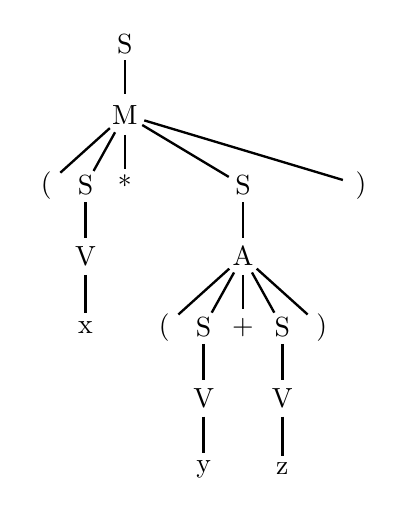
\begin{tikzpicture}[xscale=0.5,yscale=0.9,baseline={(current bounding box.center)}]
% \draw[help lines] (0,0) grid (7,2);
\node (s1) [circle,draw=none,inner sep=1pt] at (0,0) {\Snterm{S}};
{\node (s2) [circle,draw=none,inner sep=1pt] at (0,-1) {\Snterm{M}};}
{\node (s3) [circle,draw=none,inner sep=1pt] at (0,-2) {\Sterm{*}};
\node (s3a) [circle,draw=none,inner sep=1pt] at (3,-2) {\Snterm{S}};
\node (s3b) [circle,draw=none,inner sep=1pt] at (6,-2) {\Sterm{)}};
\node (s3x) [circle,draw=none,inner sep=1pt] at (-1,-2) {\Snterm{S}};
\node (s3y) [circle,draw=none,inner sep=1pt] at (-2,-2) {\Sterm{(}};}
{\node (s4) [circle,draw=none,inner sep=1pt] at (3,-3) {\Snterm{A}};}
{\node (s4z) [circle,draw=none,inner sep=1pt] at (-1,-3) {\Snterm{V}};}
{\node (s5) [circle,draw=none,inner sep=1pt] at (3,-4) {\Sterm{+}};
\node (s5a) [circle,draw=none,inner sep=1pt] at (4,-4) {\Snterm{S}};
\node (s5b) [circle,draw=none,inner sep=1pt] at (5,-4) {\Sterm{)}};
\node (s5x) [circle,draw=none,inner sep=1pt] at (2,-4) {\Snterm{S}};
\node (s5y) [circle,draw=none,inner sep=1pt] at (1,-4) {\Sterm{(}};}
{\node (s5z) [circle,draw=none,inner sep=1pt] at (-1,-4) {\Sterm{x}};}
{\node (s6a) [circle,draw=none,inner sep=1pt] at (4,-5) {\Snterm{V}};}
{\node (s6x) [circle,draw=none,inner sep=1pt] at (2,-5) {\Snterm{V}};}
{\node (s7a) [circle,draw=none,inner sep=1pt] at (4,-6) {\Sterm{z}};}
{\node (s7x) [circle,draw=none,inner sep=1pt] at (2,-6) {\Sterm{y}};}
% \node (s2) [circle,draw=none] at (0,3) {\Sterm{*}};
%
{\path[-,line width=0.3mm](s1) edge (s2);}
{\path[-,line width=0.3mm](s2) edge (s3);
\path[-,line width=0.3mm](s2) edge (s3a);
\path[-,line width=0.3mm](s2) edge (s3b);
\path[-,line width=0.3mm](s2) edge (s3x);
\path[-,line width=0.3mm](s2) edge (s3y);}
{\path[-,line width=0.3mm](s3x) edge (s4z);}
{\path[-,line width=0.3mm](s4z) edge (s5z);}
{\path[-,line width=0.3mm](s3a) edge (s4);}
{\path[-,line width=0.3mm](s4) edge (s5);
\path[-,line width=0.3mm](s4) edge (s5a);
\path[-,line width=0.3mm](s4) edge (s5b);
\path[-,line width=0.3mm](s4) edge (s5x);
\path[-,line width=0.3mm](s4) edge (s5y);}
{\path[-,line width=0.3mm](s5a) edge (s6a);}
{\path[-,line width=0.3mm](s5x) edge (s6x);}
{\path[-,line width=0.3mm](s6a) edge (s7a);}
{\path[-,line width=0.3mm](s6x) edge (s7x);}
% \path[->,line width=0.5mm](s1) edge node[below] {\Sterm{0}} (s2);
% \path[->,line width=0.5mm](s1) edge node[left] {\Sterm{1}} (s3);
% \path[->,line width=0.5mm](s3) edge node[right] {\Sterm{0}} (s2);
% \path[->,line width=0.5mm](s3) edge [loop above] node[above] {\Sterm{1}} (s3);
\end{tikzpicture}
\end{minipage}

\end{frame}


\sectionSlide{Normalisierung kontextfreier Grammatiken}

\begin{frame}\frametitle{Motivation}

Im Vergleich zu regulären Grammatiken erlauben CFGs wesentlich mehr Freiheiten bei der Formulierung von Produktionsregeln
% $\leadsto$ die selbe Sprache kann mit sehr unterschiedlichen Grammatiken ausgedrückt werden

\bigskip
\alert{Für die Angabe von Algorithmen ist es hilfreich, die Grammatik erst in eine beschränktere Form zu überführen.}
\bigskip

\examplebox{\emph{Beispiel:} Wir haben in Vorlesung~2 gezeigt, wie man $\epsilon$-Regeln in CFGs weitestgehend eliminieren kann, ohne dass sich dabei die Sprache ändert.
}

Es gibt mehrere sogenannte \redalert{Normalformen}, in die eine Grammatik durch derartige Vereinfachungen überführt werden kann.

\end{frame}

\begin{frame}\frametitle{Wiederholung: Erzeugung $\epsilon$-freier CFGs}

Der folgende Algorithmus kann $\epsilon$-Regeln eliminieren.

\codebox{
Eingabe: CFG $G=\tuple{V,\Sigma,P,S}$\\
Ausgabe: $\epsilon$-freie CFG $G'=\tuple{V',\Sigma,P',S'}$ mit $\Slang{L}(G')=\Slang{L}(G)$
% \medskip
% 
\begin{itemize}
\item Initialisiere $P' \defeq P$ und $V'\defeq V$
% 
\item Berechne $V_\epsilon = \{\Snterm{A}\in V\mid \Snterm{A}\Rightarrow^* \epsilon\}$\\ \textcolor{devilscss}{(einfaches rekursives Verfahren, siehe Vorlesung 2)}
% 
\item Entferne alle $\epsilon$-Regeln aus $P'$
% 
\item Solange es in $P'$ eine Regel $\Snterm{B}\to x\Snterm{A}y$ gibt, mit\\[1ex]
%
\narrowcentering{ $\Snterm{A}\in V_\epsilon$\hfill $|x|+|y|\geq 1$\hfill $\Snterm{B}\to xy\notin P'$ }\\[1ex]
%
wähle eine solche Regel und setze $P'\defeq P'\cup \{\Snterm{B}\to xy\}$
%
\item Falls $S\in V_\epsilon$ dann definiere ein neues Startsymbol $S'\notin V$, setze $V'\defeq V'\cup\{S'\}$ und 
$P'\defeq P'\cup\{S'\to S,S'\to\epsilon\}$.
% 
% 
% füge die Regeln
% %
% \narrowcentering{ $S'\to S$\hfill $S'\to\epsilon$ }\\[1ex]
% %
% in $P'$ ein. 
Falls $S\notin V_\epsilon$, dann verwenden wir einfach $S'\defeq S$ als Startsymbol.
\end{itemize}
}

\end{frame}

\begin{frame}\frametitle{Eliminierung von Kettenregeln}

\defbox{Eine \redalert{Kettenregel} ist eine Regel der Form $\Snterm{A}\to\Snterm{B}$.}\bigskip
\pause

\theobox{Für jede CFG $G$ gibt es eine äquivalente CFG $G'$ ohne Kettenregeln, d.h. eine CFG $G'$ für die gilt $\Slang{L}(G)=\Slang{L}(G')$.}
\pause

\emph{Beweis:} Sei $G=\tuple{V,\Sigma,P,S}$ $\epsilon$-frei (o.B.d.A.).\\$G'$ ist die Grammatik $\tuple{V,\Sigma,P',S}$, wobei sich $P'$ wie folgt ergibt: %Wir geben einen Algorithmus zur Eliminierung von Kettenregeln an.

\begin{itemize}
\item Für jedes $A\in V$ bestimmen wir rekursiv die Menge $E(A)$ aller $B\in V$, die man von $A$ aus über Kettenregeln erreichen kann:
\begin{enumerate}[(1)]
\item $A\in E(A)$
\item Falls $B\in E(A)$ und $B\to B'\in P$ mit $B'\in V$ dann $B'\in E(A)$
\end{enumerate}
{\footnotesize(Schritt (2) wird wiederholt, bis keine Änderungen mehr auftreten.)}
\item Die Produktionsregeln von $G'$ sind:
 \[P' = \bigcup_{A\in V}\Big\{ A\to w\mid \text{es gibt }B\to w\in P\text{ mit }w\notin V\text{ und }B\in E(A)\Big\}\hspace{1cm}\qed\]
%   = \bigcup_{A\in V} \bigcup_{B\in E(A)} \bigcup_{B\to w\in G\setminus G_{\text{KR}}}\{A\to w\}
\end{itemize}


\end{frame}

\begin{frame}\frametitle{Beispiel: Eliminierung von Kettenregeln}

Grammatik $G$ mit Kettenregeln:
\begin{align*}
\Snterm{S} &\to \Snterm{A}\mid \Snterm{M}\mid \Snterm{V} &
\Snterm{A} &\to \Sterm{(}\Snterm{S}\Sterm{+}\Snterm{S}\Sterm{)} &
\Snterm{M} &\to \Sterm{(}\Snterm{S}\Sterm{*}\Snterm{S}\Sterm{)} &
\Snterm{V} &\to \Sterm{x}\mid\Sterm{y}\mid\Sterm{z}
\end{align*}\vspace{-1ex}\pause

\codebox{\vspace{0ex}%
\[P' = \bigcup_{A\in V}\Big\{ A\to w\mid \text{es gibt }B\to w\in P\text{ mit }w\notin V\text{ und }B\in E(A)\Big\}\]
}\pause

Mengen erreichbarer Variablen:
\begin{align*}
E(\Snterm{S}) &=\{\Snterm{S},\Snterm{A},\Snterm{M},\Snterm{V}\} &
E(\Snterm{A}) &=\{\Snterm{A}\}& 
E(\Snterm{M}) &=\{\Snterm{M}\}&
E(\Snterm{V}) &=\{\Snterm{V}\}
\end{align*}\vspace{-1ex}\pause

Grammatik ohne Kettenregeln:
\begin{align*}
\Snterm{S} &\to \Sterm{(}\Snterm{S}\Sterm{+}\Snterm{S}\Sterm{)}\mid \Sterm{(}\Snterm{S}\Sterm{*}\Snterm{S}\Sterm{)}\mid \Sterm{x}\mid\Sterm{y}\mid\Sterm{z} \\
\Snterm{A} &\to \Sterm{(}\Snterm{S}\Sterm{+}\Snterm{S}\Sterm{)} \\
\Snterm{M} &\to \Sterm{(}\Snterm{S}\Sterm{*}\Snterm{S}\Sterm{)} \\
\Snterm{V} &\to \Sterm{x}\mid\Sterm{y}\mid\Sterm{z}
\end{align*}

\end{frame}

\begin{frame}\frametitle{Eliminierung von Kettenregeln -- Variante}

Eine verbreitete Variante bei der Eliminierung von Kettenregeln, die sich in manchen Lehrbüchern und Vorlesungsskripten findet:
\codebox{%
\begin{itemize}
\item Entferne zunächst zyklische Kettenregeln, d.h. Zyklen der Form
$B_1\to B_2, B_2\to B_3,\ldots, B_{n-1}\to B_n,B_n\to B_1$
\item Solche Zyklen kann man algorithmisch leicht finden\\ {\footnotesize(abgewandelte Version der Berechnung erreichbarer Variablen)}
\item Man kann in diesem Fall alle am Zyklus beteiligten Kettenregeln löschen und alle $B_2,\ldots,B_n$ in den übrigen Regeln durch $B_1$ ersetzten
\end{itemize}

Nach der Entfernung der Zyklen kann man die Regeln wie zuvor vereinfachen\\[1ex]
{\footnotesize
(Man spart dabei die rekursive Berechnung von $E(A)$ wenn man die Kettenregeln "`von hinten nach vorn"' eliminiert)
}
}

\end{frame}

\begin{frame}\frametitle{Die Chomsky-Normalform}

Für die algorithmische Verarbeitung kontextfreier Grammatiken ist die folgende Form besonders praktisch:

\defbox{Eine kontextfreie Grammatik $G=\tuple{V,\Sigma,P,S}$ ist in \redalert{Chomsky-Normalform} \redalert{(CNF)}, wenn alle ihre Produktionsregeln eine der beiden folgenden Formen haben:%
\[ \Snterm{A}\to \Snterm{BC} \quad\text{ (mit $\Snterm{B},\Snterm{C}\in V$)} \qquad\text{oder}\qquad \Snterm{A}\to \Sterm{c}\quad\text{ (mit $\Sterm{c}\in \Sigma$)}\]
}\pause

\theobox{\emph{Beobachtung:} Ist CFG in Chomsky-Normalform, so gilt $\epsilon\notin\Slang{L}(G)$.}

\begin{enumerate}[$\leadsto$]
\item Grammatiken, deren Sprache das leere Wort enthalten,\\ können sicher nicht in CNF sein
\item Aber wie wir wissen, gibt es in $\epsilon$-freien CFGs ohnehin höchstens eine Regel $S\to\epsilon$
\item Dieser Sonderfall kann in Algorithmen leicht berücksichtigt \ghost{werden}
\item Wir verzichten darauf, die CNF dafür noch zu erweitern
\end{enumerate}

\end{frame}

\begin{frame}[t]\frametitle{Umwandlung in CNF}

\theobox{\emph{Satz:} Für jede CFG $G$ mit $\epsilon\notin\Slang{L}(G)$ gibt es eine äquivalente CFG $\textsf{CNF}(G)$ in Chomsky-Normalform, d.h. so dass $\Slang{L}(G)=\Slang{L}(\textsf{CNF}(G))$.}\pause

\emph{Beweis: } Wir haben bereits gezeigt:
\begin{enumerate}[(1)]
\item Durch \alert{Eliminierung von $\epsilon$-Regeln} kann jede CFG in eine äquivalente $\epsilon$-freie CFG umgewandelt werden.
\item Durch \alert{Eliminierung von Kettenregeln} kann jede $\epsilon$-freie CFG in eine äquivalente CFG umgewandelt werden, in der alle Regeln die Form $\Snterm{A}\to w$ haben, mit $w\in\Sigma$ oder $|w|\geq 2$.\pause\\[1ex]
\mbox{}\hspace{-6mm}Zwei weitere Schritte führen zur Chomsky-NF:
\item \alert{Extrahiere Regeln der Form $\Snterm{A}\to\Sterm{c}$}, so dass alle anderen Regeln $\Snterm{B}\to w$
keine Terminale mehr in $w$ enthalten.
\item \alert{Zerlege Regeln der Form $\Snterm{A}\to\Sntermsub{B}{1}\cdots\Sntermsub{B}{n}$}, so dass solche Regeln
nur noch mit $n=2$ auftauchen.
\end{enumerate}

\end{frame}

\begin{frame}[t]\frametitle{Umwandlung in CNF (2)}

\theobox{\emph{Satz:} Für jede CFG $G$ mit $\epsilon\notin\Slang{L}(G)$ gibt es eine äquivalente CFG $\textsf{CNF}(G)$ in Chomsky-Normalform, d.h. so dass $\Slang{L}(G)=\Slang{L}(\textsf{CNF}(G))$.}

\emph{Beweis: } Schritt (3): \alert{Extrahiere Regeln der Form $\Snterm{A}\to\Sterm{c}$}, so dass alle anderen Regeln $\Snterm{B}\to w$ keine Terminale mehr in $w$ enthalten.\pause

\begin{itemize}
\item Führe für jedes Symbol $\Sterm{a}\in\Sigma$ eine neue Variable $\Sntermsub{V}{a}$
und eine Regel $\Sntermsub{V}{a}\to \Sterm{a}$ ein
\item Für jede Produktionsregel $\Snterm{A}\to w$ mit $|w|>1$:\\
Ersetze jedes Vorkommen eines Symbols $\Sterm{a}\in\Sigma$ in $w$ durch $\Sntermsub{V}{a}$
\end{itemize}
\emph{Anmerkungen:}\\
Regeln $\Snterm{A}\to w$ mit $|w|=0$ existieren nicht ($\epsilon$-Freiheit)\\
Regeln $\Snterm{A}\to w$ mit $|w|=1$ haben die Form $\Snterm{A}\to\Sterm{c}$ (keine \ghost{Kettenregeln)}

\end{frame}

\begin{frame}[t]\frametitle{Umwandlung in CNF (3)}

\theobox{\emph{Satz:} Für jede CFG $G$ mit $\epsilon\notin\Slang{L}(G)$ gibt es eine äquivalente CFG $\textsf{CNF}(G)$ in Chomsky-Normalform, d.h. so dass $\Slang{L}(G)=\Slang{L}(\textsf{CNF}(G))$.}

\emph{Beweis: } Schritt (4): \alert{Zerlege Regeln der Form $\Snterm{A}\to\Sntermsub{B}{1}\cdots\Sntermsub{B}{n}$}, so dass solche Regeln nur noch mit $n=2$ auftauchen.\pause
\bigskip

Für jede Produktionsregel $\Snterm{A}\to \Sntermsub{B}{1}\cdots\Sntermsub{B}{n}$ mit $n>2$:\\
\begin{itemize}
\item Führe $n-2$ neue Variablen $\Sntermsub{C}{1},\ldots,\Sntermsub{C}{n-2}$ ein
\item Ersetze die Regel durch neue Regeln:
\begin{align*}
\Snterm{A} &\to \Sntermsub{B}{1}\Sntermsub{C}{1}\\
\Sntermsub{C}{1} &\to \Sntermsub{B}{2}\Sntermsub{C}{2}\\
& \vdots\\
\Sntermsub{C}{n-3} &\to \Sntermsub{B}{n-2}\Sntermsub{C}{n-2}\\
\Sntermsub{C}{n-2} &\to \Sntermsub{B}{n-1}\Sntermsub{B}{n}
\end{align*}

% \mbox{}\hfill\ghost{\raisebox{3ex}{\qed}}
\end{itemize}

\end{frame}

\begin{frame}[t]\frametitle{Umwandlung in CNF (4)}

\theobox{\emph{Satz:} Für jede CFG $G$ mit $\epsilon\notin\Slang{L}(G)$ gibt es eine äquivalente CFG $\textsf{CNF}(G)$ in Chomsky-Normalform, d.h. so dass $\Slang{L}(G)=\Slang{L}(\textsf{CNF}(G))$.}

\emph{Beweis: } Die Korrektheit der Schritte lässt sich zeigen, indem man für eine beliebige Ableitung einer Grammatik, eine Ableitung der umgeformten Grammatik angibt. \bigskip

Zum Beispiel für Schritt 4:\\[1ex]
Eine Anwendung der Regel $\Snterm{A}\to \Sntermsub{B}{1}\cdots\Sntermsub{B}{n}$ wird dargestellt durch die
Ableitungen
\[\Snterm{A}\Rightarrow \Sntermsub{B}{1}\Sntermsub{C}{1}\Rightarrow  \Sntermsub{B}{1}\Sntermsub{B}{2}\Sntermsub{C}{2}\Rightarrow\ldots\Rightarrow\Sntermsub{B}{1}\cdots\Sntermsub{B}{n-2}\Sntermsub{C}{n-2}\Rightarrow\Sntermsub{B}{1}\cdots\Sntermsub{B}{n-2}\Sntermsub{B}{n-1}\Sntermsub{B}{n}\]
% \bigskip
% 
Korrektheit von Schritt 3 ist noch einfacher.\qed

\end{frame}

\begin{frame}\frametitle{Beispiel}

$\epsilon$-freie CFG ohne Kettenregeln:
\begin{align*}
\Snterm{S} &\to \Sterm{(}\Snterm{S}\Sterm{+}\Snterm{S}\Sterm{)}\mid \Sterm{(}\Snterm{S}\Sterm{*}\Snterm{S}\Sterm{)}\mid \Sterm{x}\mid\Sterm{y}\mid\Sterm{z}
\end{align*}

\pause Schritt (3): \alert{Extrahiere Regeln der Form $\Snterm{A}\to\Sterm{c}$}, so dass alle anderen Regeln $\Snterm{B}\to w$ keine Terminale mehr in $w$ enthalten:
%
\[\begin{array}{c}
\Snterm{S} \to \Sntermsub{V}{(}\;\Snterm{S}\;\Sntermsub{V}{+}\;\Snterm{S}\;\Sntermsub{V}{)} \mid \Sntermsub{V}{(}\;\Snterm{S}\;\Sntermsub{V}{*}\;\Snterm{S}\;\Sntermsub{V}{)} \mid \Sterm{x}\mid\Sterm{y}\mid\Sterm{z}\\
\Sntermsub{V}{(} \to \Sterm{(} \quad \Sntermsub{V}{+} \to \Sterm{+} \quad\Sntermsub{V}{)} \to \Sterm{)}\quad \Sntermsub{V}{*} \to \Sterm{*} \quad
\underbrace{\Sntermsub{V}{x} \to \Sterm{x} \quad \Sntermsub{V}{y} \to \Sterm{y} \quad\Sntermsub{V}{z} \to \Sterm{z}}_{\text{ungenutzt (dürfen entfallen)}}\\
\end{array}
\]\vspace{-1.5ex}\pause

Schritt (4): \alert{Zerlege Regeln der Form $\Snterm{A}\to\Sntermsub{B}{1}\cdots\Sntermsub{B}{n}$}, so dass solche Regeln nur noch mit $n=2$ auftauchen:
%
\[\begin{array}{c}
\Snterm{S} \to \Sntermsub{V}{(}\;\Sntermsub{C}{1} \mid \Sntermsub{V}{(}\;\Sntermsub{D}{1}\mid  \Sterm{x}\mid\Sterm{y}\mid\Sterm{z}\\
\Sntermsub{C}{1} \to \Snterm{S}\Sntermsub{C}{2} \qquad \Sntermsub{C}{2} \to \Sntermsub{V}{+}\Sntermsub{C}{3} \qquad \Sntermsub{C}{3} \to \Snterm{S}\Sntermsub{V}{)}\\
\Sntermsub{D}{1} \to \Snterm{S}\Sntermsub{D}{2} \qquad \Sntermsub{D}{2} \to \Sntermsub{V}{*}\Sntermsub{D}{3} \qquad \Sntermsub{D}{3} \to \Snterm{S}\Sntermsub{V}{)}\\
\Sntermsub{V}{(} \to \Sterm{(} \quad \Sntermsub{V}{+} \to \Sterm{+} \quad\Sntermsub{V}{)} \to \Sterm{)}\quad \Sntermsub{V}{*} \to \Sterm{*}
% \quad
% \Sntermsub{V}{x} \to \Sterm{x} \quad \Sntermsub{V}{y} \to \Sterm{y} \quad\Sntermsub{V}{z} \to \Sterm{z}
\\
\end{array}
\]

\end{frame}

\begin{frame}\frametitle{Ableitungsbäume für CNF-Grammatiken}

\alert{Besonderheit der CNF:} Alle Ableitungsbäume sind im Inneren Binärbäume und haben daher eine 
sehr reguläre Struktur\pause:
\begin{itemize}
\item Bei einem Wort $w$ der Länge $|w|$ werden genau $|w|$ Regeln vom Typ $\Snterm{A}\to\Sterm{c}$ angewendet\\
\begin{enumerate}[$\leadsto$]
\item Es gibt in der Ebene darüber genau $|w|$ Variablen
\end{enumerate}\pause
\item Jede Anwendung einer Regel vom Typ $\Snterm{A}\to\Snterm{B}\Snterm{C}$ erhöht die Anzahl der am Ende
zu ersetzenden Variablen um $1$
\begin{enumerate}[$\leadsto$]
\item für ein Wort der Länge $|w|$ müssen genau $|w|-1$ Regeln vom Typ $\Snterm{A}\to\Snterm{B}\Snterm{C}$ angewendet werden
\end{enumerate}
\end{itemize}\pause
Wir folgern:

\theobox{\emph{Satz:} Wenn $w\in\Slang{L}(G)$ für eine Grammatik $G$ in CNF, dann hat jede Ableitung für $w$ genau $2|w|-1$ Ableitungsschritte.}

\end{frame}

\sectionSlide{Das Wortproblem für CFGs}

\begin{frame}\frametitle{Das Wortproblem für CFGs}

\defbox{
Das \redalert{Wortproblem} für eine Sprache $\Slang{L}$ über Alphabet $\Sigma$ besteht darin, die folgende Funktion zu berechnen:\\[1ex]
\emph{Eingabe:} ein Wort $w\in\Sigma^*$\\
\emph{Ausgabe:} "`ja"' wenn $w\in\Slang{L}$ und "`nein"' wenn $w\notin\Slang{L}$
}\pause

Für Typ-2-Sprachen $\Slang{L}$ können wir bereits ein (schlechtes) Entscheidungsverfahren angeben:
\begin{itemize}
\item Es gibt eine CFG für $\Slang{L}$
\item Also gibt es eine CNF für $\Slang{L}$
\item Also hat jedes Wort $w\in\Slang{L}$ eine Ableitung der Länge $2|w|-1$
\item Wir können systematisch alle Ableitungen dieser Länge betrachten und prüfen, ob eine davon $w$ erzeugt
\end{itemize}\pause
$\leadsto$ exponentieller Algorithmus
\bigskip

\narrowcentering{\alert{Geht es auch besser?}}

\end{frame}

\begin{frame}\frametitle{Sakai, Kasami, Younger, Cocke und Schwartz}

Verschiedene Menschen fanden eine bessere Lösung:
\begin{itemize}
\item Itiroo Sakai, 1961: "`Syntax in universal translation"'
\item Tadao Kasami, 1965: "`An efficient recognition and syntax-analysis algorithm for context-free languages"'
\item Daniel H. Younger, 1967: "`Recognition and parsing of context-free languages in time $n^3$"'
\item John Cocke, Jacob T. Schwartz, 1970: "`Programming languages and their compilers"'
\end{itemize}
% Cocke ist "der Vater der RISC-Architektur" und Turing-Award-Gewinner
% Die Version von Itiroo Sakai ist vermutlich etwas implizit, da Kasami oft als der erste genannt wird
% Es ist unklar, warum Schwartz nicht aufgefuehrt wird in CYK
\bigskip

\alert{Das Ergebnis ist bekannt als CYK-Algorithmus (Cocke-Younger-Kasami).}

\end{frame}

\newcommand{\Rightarrowstarquest}{\mathrel{{\stackrel{?}{\Rightarrow}}{}^*}}

\begin{frame}\frametitle{CYK: Grundidee}

Der CYK-Algorithmus arbeitet mit einer kontextfreien Grammatik $G$ in CNF.
\bigskip

\alert{Wie kann man prüfen, ob ein Wort $w=\Sterm{a_1}\cdots\Sterm{a_n}$ durch so eine Grammatik abgeleitet werden kann?}
\pause

\begin{itemize}
\item Falls $|w|=1$, dann ist $w\in\Sigma$ und es gilt:\\
$w\in\Slang{L}(G)$ genau dann wenn es eine Regel $\Snterm{S}\to w$ in $G$ gibt\pause
\item Falls $|w|>1$, dann ist:\\
$w\in\Slang{L}(G)$ genau dann wenn es eine Regel
$\Snterm{S}\to\Snterm{A}\Snterm{B}$ und eine Zahl $i$ gibt, so dass gilt
\[\Snterm{A}\Rightarrow^* \Sterm{a_1}\cdots\Sterm{a_i}\qquad\text{und}\qquad \Snterm{B}\Rightarrow^* \Sterm{a_{i+1}}\cdots\Sterm{a_n}\]
\end{itemize}\pause

\emph{Idee:} Fall 2 reduziert das Problem $\Snterm{S}\Rightarrowstarquest w$ auf zwei einfachere Probleme
$\Snterm{A}\Rightarrowstarquest \Sterm{a_1}\cdots\Sterm{a_i}$ und $\Snterm{B}\Rightarrowstarquest \Sterm{a_{i+1}}\cdots\Sterm{a_n}$, die man allerdings für alle Regeln $\Snterm{S}\to\Snterm{A}\Snterm{B}$ und Indizes $i$ lösen muss

\end{frame}

\begin{frame}\frametitle{CYK: Praktische Umsetzung}

\anybox{purple}{Notation: Für $w=\Sterm{a_1}\cdots\Sterm{a_n}$ schreiben wir $w_{i,j}$ für das
Teilwort $\Sterm{a_i}\cdots\Sterm{a_{j}}$, also das Infix der Länge $j-i+1$, welches an Position $i$ beginnt.
}

\emph{Vorgehen:} Wir berechnen für jedes Teilwort $w_{i,j}$ die Menge aller Variablen $\Snterm{A}$, für
die gilt $\Snterm{A}\Rightarrow^* w_{i,j}$. Diese Menge nennen wir $V[i,j]$.
\begin{itemize}
\item Wir beginnen mit den kürzesten Teilwörtern ($i=j$)
\item Für längere Wörter betrachten wir jede mögliche Zweiteilung $w_{i,j}=w_{i,k}w_{k+1,j}$ und suchen Regeln der Form $\Snterm{A}\to\Snterm{B}\Snterm{C}$ so dass $\Snterm{B}\in V[i,k]$ und $\Snterm{C}\in V[k+1,j]$
\end{itemize}
Ist am Ende das Startsymbol $S\in V[1,|w|]$, dann liegt $w$ in der Sprache

\end{frame}

\newcommand{\MEC}[1]{\multicolumn{1}{c}{#1}}
\begin{frame}\frametitle{Notation}

% Je größer $i$, desto kürzer die mögliche Wortlänge $\ell$, denn $i+\ell \leq |w|$\\
Für die Teilwörter $w_{i,j}$ gilt $i\leq j$\\
$\leadsto$ Die Mengen $V[i,j]$ können als Dreiecksmatrix notiert werden
\bigskip

\emph{Beispiel:} Wir betrachten das Wort $w=\Sterm{a+b*c}$ der Länge $|w|=5$.\bigskip

Darstellung der Mengen $V[i,j]$:\bigskip

\narrowcentering{%
\begin{tabular}{c|c|c|c|c|c|}
%  \multicolumn{1}{c}{}  & \multicolumn{1}{c}{A} & \multicolumn{1}{c}{B} & \multicolumn{1}{c}{C} & \multicolumn{1}{c}{D}  \\\cline{2-5}
\cline{2-6}
\Sterm{a}
	& $V[1,1]$ & $V[1,2]$ & $V[1,3]$ & $V[1,4]$ & $V[1,5]$ \\\cline{2-6}
\MEC{\Sterm{+}} &  
	           & $V[2,2]$ & $V[2,3]$ & $V[2,4]$ & $V[2,5]$ \\\cline{3-6}
 \MEC{\Sterm{b}} &\MEC{}   &
	                      & $V[3,3]$ & $V[3,4]$ & $V[3,5]$ \\\cline{4-6}
 \MEC{\Sterm{*}} &\MEC{}   &\MEC{}   &   
	                                 & $V[4,4]$ & $V[4,5]$ \\\cline{5-6}
 \MEC{\Sterm{c}} &\MEC{}   &\MEC{}   &\MEC{}   &
	                                            & $V[5,5]$ \\\cline{6-6}
 \MEC{}          &\MEC{\Sterm{a}} & \MEC{\Sterm{+}} & \MEC{\Sterm{b}} & \MEC{\Sterm{*}} & \MEC{\Sterm{c}}
\end{tabular}}

\end{frame}

\newcommand{\hicell}[1]{\only<#1|handout:0>{\cellcolor{strongyellow}}}
\newcommand{\upcell}[2]{\only<#1|handout:0>{\cellcolor{strongyellow}}\visible<#1->{#2}}
\newcommand{\locell}[1]{\only<#1|handout:0>{\cellcolor{darkgreen!20}}}

\begin{frame}\frametitle{Beispiel}

Grammatik:\\[1ex]
$
\Snterm{S}\to \Snterm{S}\Snterm{A}\mid \Snterm{S}\Snterm{M} \mid \Sterm{a}\mid \Sterm{b}\mid \Sterm{c}$\\
$\Snterm{A}\to \Snterm{P}\Snterm{S} \qquad \Snterm{M} \to \Snterm{T}\Snterm{S}\qquad
\Snterm{P}\to \Sterm{+} \qquad \Snterm{T} \to \Sterm{*}
% \\
% \Snterm{N} \to \Snterm{P}\Snterm{Z}\qquad \Snterm{Z}\to \Sterm{a}\mid \Sterm{b}\mid \Sterm{c}
$\\[2ex]
Wort: $w=\Sterm{a+b*c}$
\bigskip

Berechnung der Mengen $V[i,j]$:\bigskip

\narrowcentering{%
\begin{tabular}{c|c|c|c|c|c|}
%  \multicolumn{1}{c}{}  & \multicolumn{1}{c}{A} & \multicolumn{1}{c}{B} & \multicolumn{1}{c}{C} & \multicolumn{1}{c}{D}  \\\cline{2-5}
\cline{2-6}
\Sterm{a}
	& \hicell{2}\upcell{3}{$\Snterm{S}$}\locell{10,20,21,31,40-41}
		& \hicell{9,10}\locell{22,32,42}
			& \hicell{19,20,22}\upcell{21}{$\Snterm{S}$}\locell{33,43}
				& \hicell{30-33}\locell{44}
					& \hicell{39-43}\upcell{41}{$\Snterm{S}$} \\\cline{2-6}
\MEC{\Sterm{+}} &  
		& \hicell{4}\upcell{5}{$\Snterm{P}$}\locell{10,12-13,24,35-36}
			& \hicell{11,12}\upcell{13}{$\Snterm{A}$}\locell{20-21,25,37}
				& \hicell{23-25}\locell{31,38}
					& \hicell{34-38}\upcell{36}{$\Snterm{A}$}\locell{40-41} \\\cline{3-6}
 \MEC{\Sterm{b}} &\MEC{}   &
			& \upcell{6}{$\Snterm{S}$}\locell{12,13,15,22,27-28}
				&  \hicell{14,15}\locell{24,29,32}
					& \hicell{26-29}\upcell{28}{$\Snterm{S}$}\locell{35-36,42} \\\cline{4-6}
 \MEC{\Sterm{*}} &\MEC{}   &\MEC{}   &   
				& \upcell{7}{$\Snterm{T}$}\locell{15,17,18,25,33}
					& \hicell{16,17}\upcell{18}{$\Snterm{M}$}\locell{27-28,37,43} \\\cline{5-6}
 \MEC{\Sterm{c}} &\MEC{}   &\MEC{}   &\MEC{}   &
					& \upcell{8}{$\Snterm{S}$}\locell{17,18,29,38,44} \\\cline{6-6}
 \MEC{}          &\MEC{\Sterm{a}} & \MEC{\Sterm{+}} & \MEC{\Sterm{b}} & \MEC{\Sterm{*}} & \MEC{\Sterm{c}}
\end{tabular}}\bigskip

\narrowcentering{\visible<45->{$S\in V[1,5]$ $\leadsto$ \redalert{$w$ kann erzeugt werden}}}

\end{frame}

\begin{frame}\frametitle{Der CYK-Algorithmus}

\codebox{
\emph{Eingabe:} Wort $w=\Sterm{a_1}\cdots\Sterm{a_n}$, CNF-Grammatik $G=\tuple{V,\Sigma,P, \Snterm{S}}$\\
\emph{Ausgabe:} "`ja"' wenn $w\in\Slang{L}(G)$; sonst "`nein"'\\[1ex]
%
% Grundfall:\\
\emph{for} $i=1,\ldots,n$:~~~\textcolor{devilscss}{// Teilwörter der Länge 1}\\
~~~$V[i,i]\defeq \{\Snterm{A}\in V\mid \Snterm{A}\to\Sterm{a_i}\in P\}$\\[2ex]
\emph{for} $d=1,\ldots,n-1$:~~~\textcolor{devilscss}{// Differenz Endindex $-$ Startindex}\\
~~~\emph{for} $i=1,\ldots,n-d$:~~~\textcolor{devilscss}{// Startindex}\\
~~~~~~$j\defeq i+d$\\
~~~~~~$V[i,j]\defeq \emptyset$\\
~~~~~~\emph{for} $k=i,\ldots,j-1$:~~~\textcolor{devilscss}{// Trennindex}\\
~~~~~~~~~$V[i,j]\defeq V[i,j]\cup \{\Snterm{A}\in V\mid \text{es gibt }\Snterm{A}\to\Snterm{B}\Snterm{C}\in P\text{ mit}$\\
~~~~~~~~~\hspace{3.8cm}$\Snterm{B}\in V[i,k]\text{ und }\Snterm{C}\in V[k+1,j]\}$\\[2ex]
\emph{return} $\Snterm{S}\in V[1,n]$ \emph{?} "`ja"' \emph{:} "`nein"'
}

\end{frame}

\begin{frame}\frametitle{Bezug zur Tabelle}

\scalebox{0.7}{%
\begin{minipage}{8cm}\codebox{
\emph{Eingabe:} Wort $w=\Sterm{a_1}\cdots\Sterm{a_n}$,\\
\hspace{2cm}CNF-Grammatik $G=\tuple{V,\Sigma,P, \Snterm{S}}$\\
\emph{Ausgabe:} "`ja"' wenn $w\in\Slang{L}(G)$; sonst "`nein"'\\[1ex]
%
% Grundfall:\\
\ghost{\hspace{8.3cm}{\huge$\Leftarrow$}
\begin{tabular}{c|c|c|c|c|c|}
%  \multicolumn{1}{c}{}  & \multicolumn{1}{c}{A} & \multicolumn{1}{c}{B} & \multicolumn{1}{c}{C} & \multicolumn{1}{c}{D}  \\\cline{2-5}
\cline{2-6}
\Sterm{a}
	& \cellcolor{purple!20}  &   &   &   &   \\\cline{2-6}
\MEC{\Sterm{+}} &  
	& \cellcolor{purple!40}  &   &   &   \\\cline{3-6}
 \MEC{\Sterm{b}} &\MEC{}   &
	& \cellcolor{purple!60}  &   &   \\\cline{4-6}
 \MEC{\Sterm{*}} &\MEC{}   &\MEC{}   &   
	& \cellcolor{purple!80}  &  \\\cline{5-6}
 \MEC{\Sterm{c}} &\MEC{}   &\MEC{}   &\MEC{}   &
	& \cellcolor{purple!100}  \\\cline{6-6}
 \MEC{}          &\MEC{\Sterm{a}} & \MEC{\Sterm{+}} & \MEC{\Sterm{b}} & \MEC{\Sterm{*}} & \MEC{\Sterm{c}}
\end{tabular}
}%
\emph{for} $i=1,\ldots,n$:~~~\textcolor{devilscss}{// Teilwörter der Länge 1}\\
~~~$V[i,i]\defeq \{\Snterm{A}\in V\mid \Snterm{A}\to\Sterm{a_i}\in P\}$\\[2ex]
\emph{for} $d=1,\ldots,n-1$:~~~\textcolor{devilscss}{// Differenz Endind. $-$ Startind.}\\
~~~\emph{for} $i=1,\ldots,n-d$:~~~\textcolor{devilscss}{// Startindex}\\
~~~~~~$j\defeq i+d$\\
~~~~~~$V[i,j]\defeq \emptyset$\\
~~~~~~\emph{for} $k=i,\ldots,j-1$:~~~\textcolor{devilscss}{// Trennindex}\\
~~~~~~~~~$V[i,j]\defeq V[i,j]\cup{}$\\
~~~~~~~~~\hspace{1.4cm}$\{\Snterm{A}\in V\mid \text{es gibt }\Snterm{A}\to\Snterm{B}\Snterm{C}\in P\text{ mit}$\\
~~~~~~~~~\hspace{2cm}$\Snterm{B}\in V[i,k]\text{ und }\Snterm{C}\in V[k+1,j]\}$\\[2ex]
\emph{return} $\Snterm{S}\in V[1,n]$ \emph{?} "`ja"' \emph{:} "`nein"'
}\end{minipage}}

\end{frame}

\begin{frame}\frametitle{Bezug zur Tabelle}

\scalebox{0.7}{%
\begin{minipage}{8cm}\codebox{
\emph{Eingabe:} Wort $w=\Sterm{a_1}\cdots\Sterm{a_n}$,\\
\hspace{2cm}CNF-Grammatik $G=\tuple{V,\Sigma,P, \Snterm{S}}$\\
\emph{Ausgabe:} "`ja"' wenn $w\in\Slang{L}(G)$; sonst "`nein"'\\[1ex]
%
% Grundfall:\\
\emph{for} $i=1,\ldots,n$:~~~\textcolor{devilscss}{// Teilwörter der Länge 1}\\
~~~$V[i,i]\defeq \{\Snterm{A}\in V\mid \Snterm{A}\to\Sterm{a_i}\in P\}$\\[2ex]
\ghost{\hspace{8.3cm}{\huge$\Leftarrow$}
\begin{tabular}{c|c|c|c|c|c|}
%  \multicolumn{1}{c}{}  & \multicolumn{1}{c}{A} & \multicolumn{1}{c}{B} & \multicolumn{1}{c}{C} & \multicolumn{1}{c}{D}  \\\cline{2-5}
\cline{2-6}
\Sterm{a}
	&  & \cellcolor{purple!20}   & \cellcolor{purple!40}   & \cellcolor{purple!60}  & \cellcolor{purple!80}  \\\cline{2-6}
\MEC{\Sterm{+}} &  
	&  & \cellcolor{purple!20}   & \cellcolor{purple!40}  &  \cellcolor{purple!60} \\\cline{3-6}
 \MEC{\Sterm{b}} &\MEC{}   &
	&  & \cellcolor{purple!20}   & \cellcolor{purple!40}  \\\cline{4-6}
 \MEC{\Sterm{*}} &\MEC{}   &\MEC{}   &   
	&  & \cellcolor{purple!20}  \\\cline{5-6}
 \MEC{\Sterm{c}} &\MEC{}   &\MEC{}   &\MEC{}   &
	&  \\\cline{6-6}
 \MEC{}          &\MEC{\Sterm{a}} & \MEC{\Sterm{+}} & \MEC{\Sterm{b}} & \MEC{\Sterm{*}} & \MEC{\Sterm{c}}
\end{tabular}
}%
\emph{for} $d=1,\ldots,n-1$:~~~\textcolor{devilscss}{// Differenz Endind. $-$ Startind.}\\
~~~\emph{for} $i=1,\ldots,n-d$:~~~\textcolor{devilscss}{// Startindex}\\
~~~~~~$j\defeq i+d$\\
~~~~~~$V[i,j]\defeq \emptyset$\\
~~~~~~\emph{for} $k=i,\ldots,j-1$:~~~\textcolor{devilscss}{// Trennindex}\\
~~~~~~~~~$V[i,j]\defeq V[i,j]\cup{}$\\
~~~~~~~~~\hspace{1.4cm}$\{\Snterm{A}\in V\mid \text{es gibt }\Snterm{A}\to\Snterm{B}\Snterm{C}\in P\text{ mit}$\\
~~~~~~~~~\hspace{2cm}$\Snterm{B}\in V[i,k]\text{ und }\Snterm{C}\in V[k+1,j]\}$\\[2ex]
\emph{return} $\Snterm{S}\in V[1,n]$ \emph{?} "`ja"' \emph{:} "`nein"'
}\end{minipage}}

\end{frame}

\begin{frame}\frametitle{Bezug zur Tabelle}

\scalebox{0.7}{%
\begin{minipage}{8cm}\codebox{
\emph{Eingabe:} Wort $w=\Sterm{a_1}\cdots\Sterm{a_n}$,\\
\hspace{2cm}CNF-Grammatik $G=\tuple{V,\Sigma,P, \Snterm{S}}$\\
\emph{Ausgabe:} "`ja"' wenn $w\in\Slang{L}(G)$; sonst "`nein"'\\[1ex]
%
% Grundfall:\\
\emph{for} $i=1,\ldots,n$:~~~\textcolor{devilscss}{// Teilwörter der Länge 1}\\
~~~$V[i,i]\defeq \{\Snterm{A}\in V\mid \Snterm{A}\to\Sterm{a_i}\in P\}$\\[2ex]
\emph{for} $d=1,\ldots,n-1$:~~~\textcolor{devilscss}{// Differenz Endind. $-$ Startind.}\\
\ghost{\hspace{8.3cm}{\huge$\Leftarrow$}
\begin{tabular}{c|c|c|c|c|c|}
%  \multicolumn{1}{c}{}  & \multicolumn{1}{c}{A} & \multicolumn{1}{c}{B} & \multicolumn{1}{c}{C} & \multicolumn{1}{c}{D}  \\\cline{2-5}
\cline{2-6}
\Sterm{a}
	&  & \cellcolor{purple!20}  &   &   &   \\\cline{2-6}
\MEC{\Sterm{+}} &  
	&  & \cellcolor{purple!40}  &   &   \\\cline{3-6}
 \MEC{\Sterm{b}} &\MEC{}   &
	&  & \cellcolor{purple!60}  &   \\\cline{4-6}
 \MEC{\Sterm{*}} &\MEC{}   &\MEC{}   &   
	&  & \cellcolor{purple!80} \\\cline{5-6}
 \MEC{\Sterm{c}} &\MEC{}   &\MEC{}   &\MEC{}   &
	&  \\\cline{6-6}
 \MEC{}          &\MEC{\Sterm{a}} & \MEC{\Sterm{+}} & \MEC{\Sterm{b}} & \MEC{\Sterm{*}} & \MEC{\Sterm{c}}
\end{tabular}
}%
~~~\emph{for} $i=1,\ldots,n-d$:~~~\textcolor{devilscss}{// Startindex}\\
~~~~~~$j\defeq i+d$\\
~~~~~~$V[i,j]\defeq \emptyset$\\
~~~~~~\emph{for} $k=i,\ldots,j-1$:~~~\textcolor{devilscss}{// Trennindex}\\
~~~~~~~~~$V[i,j]\defeq V[i,j]\cup{}$\\
~~~~~~~~~\hspace{1.4cm}$\{\Snterm{A}\in V\mid \text{es gibt }\Snterm{A}\to\Snterm{B}\Snterm{C}\in P\text{ mit}$\\
~~~~~~~~~\hspace{2cm}$\Snterm{B}\in V[i,k]\text{ und }\Snterm{C}\in V[k+1,j]\}$\\[2ex]
\emph{return} $\Snterm{S}\in V[1,n]$ \emph{?} "`ja"' \emph{:} "`nein"'
}\end{minipage}}

\end{frame}


\begin{frame}\frametitle{Bezug zur Tabelle}

\scalebox{0.7}{%
\begin{minipage}{8cm}\codebox{
\emph{Eingabe:} Wort $w=\Sterm{a_1}\cdots\Sterm{a_n}$,\\
\hspace{2cm}CNF-Grammatik $G=\tuple{V,\Sigma,P, \Snterm{S}}$\\
\emph{Ausgabe:} "`ja"' wenn $w\in\Slang{L}(G)$; sonst "`nein"'\\[1ex]
%
% Grundfall:\\
\emph{for} $i=1,\ldots,n$:~~~\textcolor{devilscss}{// Teilwörter der Länge 1}\\
~~~$V[i,i]\defeq \{\Snterm{A}\in V\mid \Snterm{A}\to\Sterm{a_i}\in P\}$\\[2ex]
\emph{for} $d=1,\ldots,n-1$:~~~\textcolor{devilscss}{// Differenz Endind. $-$ Startind.}\\
~~~\emph{for} $i=1,\ldots,n-d$:~~~\textcolor{devilscss}{// Startindex}\\
~~~~~~$j\defeq i+d$\\
~~~~~~$V[i,j]\defeq \emptyset$\\
\ghost{\hspace{8.3cm}{\huge$\Leftarrow$}
\begin{tabular}{c|c|c|c|c|c|}
%  \multicolumn{1}{c}{}  & \multicolumn{1}{c}{A} & \multicolumn{1}{c}{B} & \multicolumn{1}{c}{C} & \multicolumn{1}{c}{D}  \\\cline{2-5}
\cline{2-6}
\Sterm{a}
	&  &   &   &   &   \\\cline{2-6}
\MEC{\Sterm{+}} &  
	& \cellcolor{purple!20} & \cellcolor{purple!50}  & \cellcolor{purple!80}  &   \\\cline{3-6}
 \MEC{\Sterm{b}} &\MEC{}   &
	&  &   &  \cellcolor{purple!20} \\\cline{4-6}
 \MEC{\Sterm{*}} &\MEC{}   &\MEC{}   &   
	&  & \cellcolor{purple!50} \\\cline{5-6}
 \MEC{\Sterm{c}} &\MEC{}   &\MEC{}   &\MEC{}   &
	& \cellcolor{purple!80} \\\cline{6-6}
 \MEC{}          &\MEC{\Sterm{a}} & \MEC{\Sterm{+}} & \MEC{\Sterm{b}} & \MEC{\Sterm{*}} & \MEC{\Sterm{c}}
\end{tabular}
}%
~~~~~~\emph{for} $k=i,\ldots,j-1$:~~~\textcolor{devilscss}{// Trennindex}\\
~~~~~~~~~$V[i,j]\defeq V[i,j]\cup{}$\\
~~~~~~~~~\hspace{1.4cm}$\{\Snterm{A}\in V\mid \text{es gibt }\Snterm{A}\to\Snterm{B}\Snterm{C}\in P\text{ mit}$\\
~~~~~~~~~\hspace{2cm}$\Snterm{B}\in V[i,k]\text{ und }\Snterm{C}\in V[k+1,j]\}$\\[2ex]
\emph{return} $\Snterm{S}\in V[1,n]$ \emph{?} "`ja"' \emph{:} "`nein"'
}\end{minipage}}

\end{frame}

\begin{frame}\frametitle{Komplexität}

\alert{Wie komplex ist der CYK-Algorithmus?}
\begin{itemize}
\item Drei geschachtelte Schleifen mit Lauflänge $O(|w|)$
\item Operationen für Zugriff auf Grammatik und Teilmengen von $V$:%
\begin{itemize}
\item polynomiell bezüglich der Größe der Grammatik
\item konstant wenn die Grammatik vorher bekannt und fest ist
\end{itemize}
\end{itemize}\bigskip

\theobox{\emph{Satz:} Das Wortproblem für kontextfreie Sprachen ist in $O(n^3)$ lösbar.}\bigskip

\emph{Anmerkung:} Die Umwandlung in CNF verlangt $\epsilon\notin\Slang{L}(G)$, aber 
im Fall $\epsilon\in\Slang{L}(G)$ kann man eine Grammatik $G'$ mit $\epsilon\notin\Slang{L}(G')$ erzeugen und
$w=\epsilon$ gesondert testen.

\end{frame}


\begin{frame}\frametitle{Zusammenfassung und Ausblick}

Jede Typ-2-Grammatik kann in eine äquivalente$^*$ Grammatik in \redalert{Chomsky-Normalform} umgewandelt werden.\\
{\tiny $^*$ besser: äquivalent bis auf das leere Wort, welches von der normalisierten Grammatik nicht erzeugt wird}
\bigskip

Mithilfe des \redalert{CYK-Algorithmus} ist das Wortproblem für kontextfreie Sprachen in polynomieller Zeit lösbar
\bigskip

\anybox{yellow}{
Offene Fragen:
\begin{itemize}
\item Haben kontextfreie Sprachen ein Berechnungsmodell?
\item Wie sehen nichtkontextfreie Sprachen aus und wie erkennt man sie?
\end{itemize}
}

\end{frame}


\end{document}
